Lurking behind WEKA's interactive interfaces---the Explorer, the
Knowledge Flow, the Experimenter and the Workbench---lies its basic
functionality. This can be accessed more directly through a
command-line interface. Select \textit{Simple CLI} from the interface
choices at the right of Figure~\ref{subfig:explorer_1} to bring up a
plain textual panel with a line at the bottom on which you enter
commands. Alternatively, use the operating system's command-line
interface to run the classes in \textit{weka.jar}, in which case you
must first set the \textit{CLASSPATH} environment variable as
explained in WEKA's \textit{README} file.

\section{Getting started}

At the beginning of Section~\ref{subsection:building_decision_tree} we
used the Explorer to invoke the J4.8 learner on the weather data. To
do the same thing in the command-line interface, type

\begin{Verbatim}[fontsize=\footnotesize]
java weka.classifiers.trees.J48 -t data/weather.arff
\end{Verbatim}

\noindent into the line at the bottom of the text panel. This
incantation calls the Java virtual machine (in the Simple CLI, Java is
already loaded) and instructs it to execute J4.8. WEKA is organized in
\textit{packages} (not to be confused with the plugin packages that
are managed by WEKA's package manager) that correspond to a directory
hierarchy. The program to be executed is called \textit{J48} and
resides in the \textit{trees} package, which is a subpackage of
\textit{classifiers}, which is part of the overall weka package. The
next section gives more details of the package structure. The
\textit{--t} option signals that the next argument is the name of the
training file: we are assuming that the weather data resides in a
\textit{data} subdirectory of the directory from which you fired up
WEKA. The result resembles the text shown in
Figure~\ref{fig:j48_output}. In the Simple CLI it appears in the panel
above the line where you typed the command.

\subsection{weka.Run}

Typing in fully qualified class names can become a chore after a
while, especially if you are using meta learning schemes that
themselves require various base learners to be specified. Using the
\textit{weka.Run} command line tool allows you to type in shortened versions of
scheme names, and WEKA will attempt to find a match by scanning the
names of all the schemes it knows about. Using weka.Run, the previous
J4.8 invocation becomes

\begin{Verbatim}[fontsize=\footnotesize]
java weka.Run .J48 -t data/weather.arff
\end{Verbatim}

\noindent A small saving perhaps, but consider the following

\begin{Verbatim}[fontsize=\footnotesize]
java weka.Run .Stacking -M .Logistic -B .J48 -B ".FilteredClassifier -F \".Remove -R 1\" 
  -W .NaiveBayes" -B .OneR -t data/iris.arff
\end{Verbatim}

\noindent Without weka.Run's scheme matching this would look like

\begin{Verbatim}[fontsize=\footnotesize]
java weka.classifiers.meta.Stacking -M weka.classifiers.functions.Logistic 
  -B weka.classifiers.trees.J48 -B "weka.classifiers.meta.FilteredClassifier 
  -F \"weka.filters.unsupervised.attribute.Remove -R 1\" 
  -W weka.classifiers.bayes.NaiveBayes" -B weka.classifiers.rules.OneR 
  -t data/iris.arff
\end{Verbatim}

\noindent If you are not using the Simple CLI, but instead are using
your operating system's command-line interface, then weka.Run provides
another benefit---it automatically adds all the classes from plugin
packages into the CLASSPATH. This saves having to modify the CLASSPATH
every time you install a new plugin package.

\section{The structure of WEKA}

We have explained how to invoke filtering and learning schemes with
the Explorer and connect them together with the Knowledge Flow
interface. To go further, it is necessary to learn something about how
WEKA is put together. Detailed, up-to-date information can be found in
the online documentation included in the distribution. This is more
technical than the descriptions of the learning and filtering schemes
given by the \textit{More} button in the Explorer and Knowledge Flow's
object editors. It is generated directly from comments in the source
code using Sun's Javadoc utility. To understand its structure, you
need to know how Java programs are organized.

\subsection{Classes, instances, and packages}

Every Java program is implemented as a class or collection of
classes. In object-oriented programming, a \textit{class} is a
collection of variables along with some \textit{methods} that operate
on them. Together, they define the behavior of an object belonging to
the class. An \textit{object} is simply an instantiation of the class
that has values assigned to all the class's variables. In Java, an
object is also called an \textit{instance} of the
class. Unfortunately, this conflicts with the terminology used in this
book, where the terms \textit{class} and \textit{instance} appear in
the quite different context of machine learning. From now on, you will
have to infer the intended meaning of these terms from their
context. This is not difficult---and sometimes we'll use the word object
instead of Java's instance to make things clear.

In WEKA, the implementation of a particular learning algorithm is
encapsulated in a class---which may depend on other classes for some
of its functionality. For example, the \textit{J48} class described
previously builds a C4.5 decision tree. Each time the Java virtual
machine executes \textit{J48}, it creates an instance of this class by
allocating memory for building and storing a decision tree
classifier. The algorithm, the classifier it builds, and a procedure
for outputting the classifier are all part of that instantiation of
the \textit{J48} class.

Larger programs are usually split into more than one class. The
\textit{J48} class, for example, does not actually contain any code
for building a decision tree. It includes references to instances of
other classes that do most of the work. When there are a lot of
classes---as in WEKA---they become difficult to comprehend and
navigate. Java allows classes to be organized into packages. A
\textit{package} is just a directory containing a collection of
related classes: for example, the \textit{trees} package mentioned
previously contains the classes that implement decision
trees. Packages are organized in a hierarchy that corresponds to the
directory hierarchy: \textit{trees} is a subpackage of the
\textit{classifiers} package, which is itself a subpackage of the
overall \textit{weka} package.

\begin{figure}[!thp]
\centering
\subfloat{\label{subfig:javadoc_a_1}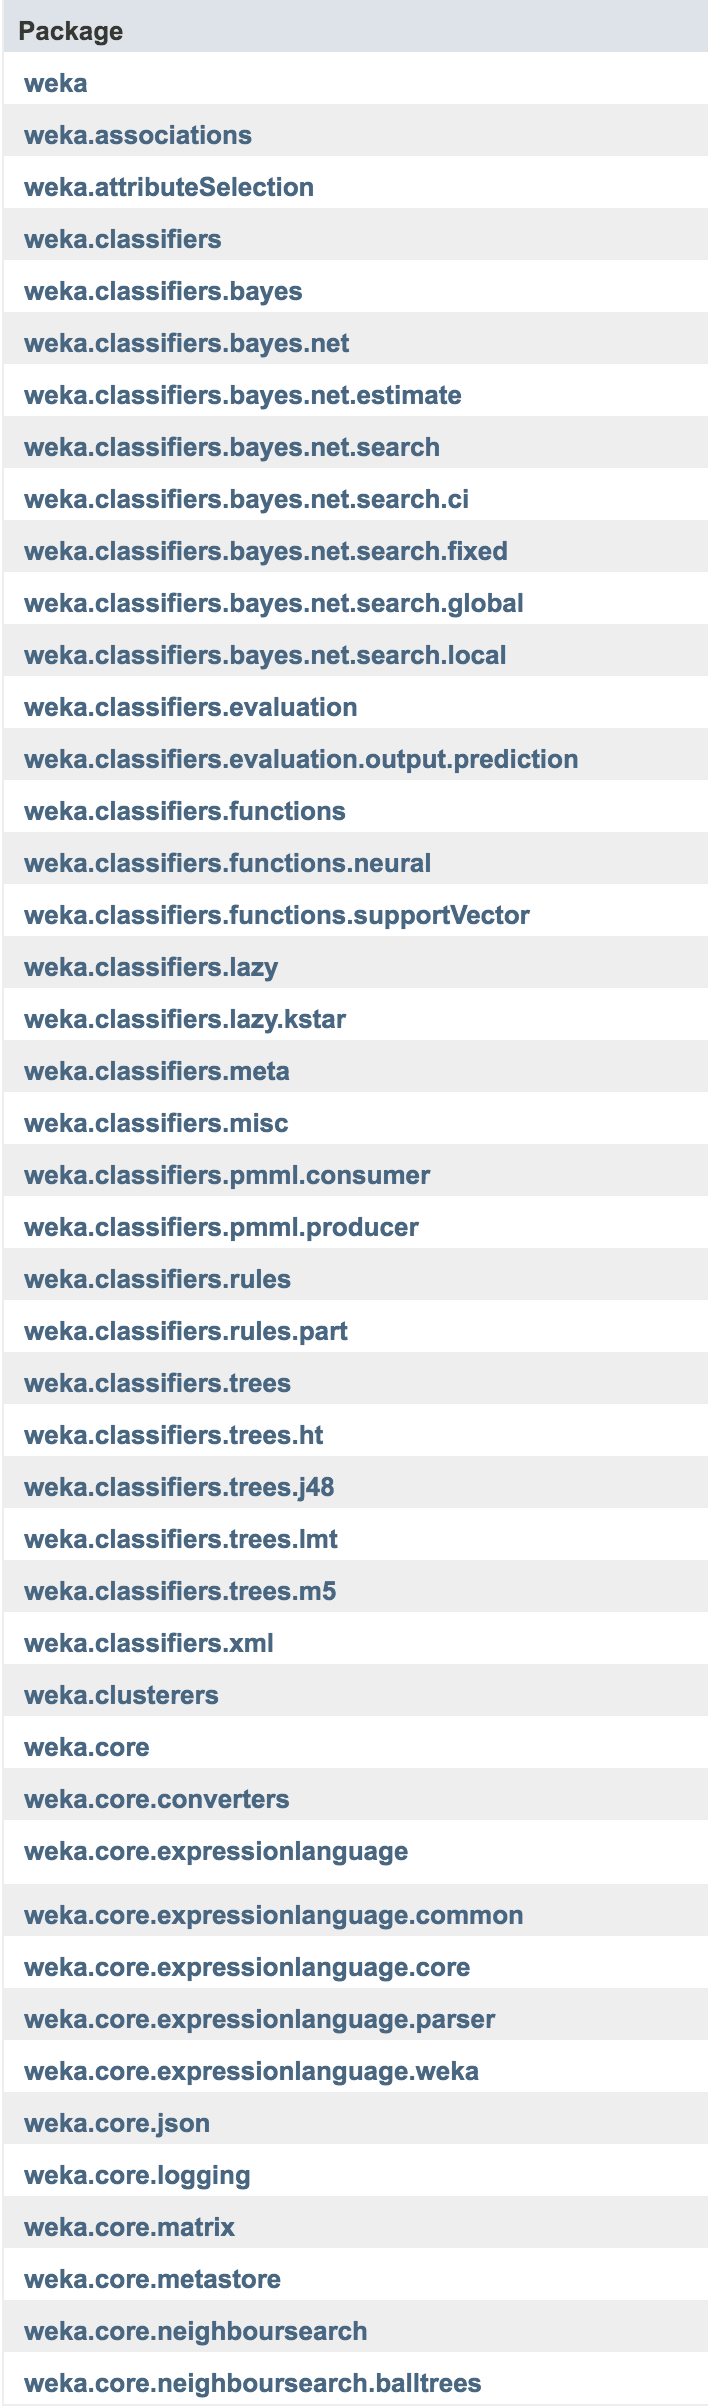
\includegraphics[width=0.45\textwidth]{images/B5_1a1.png}}
\qquad
\subfloat{\label{subfig:javadoc_a_2}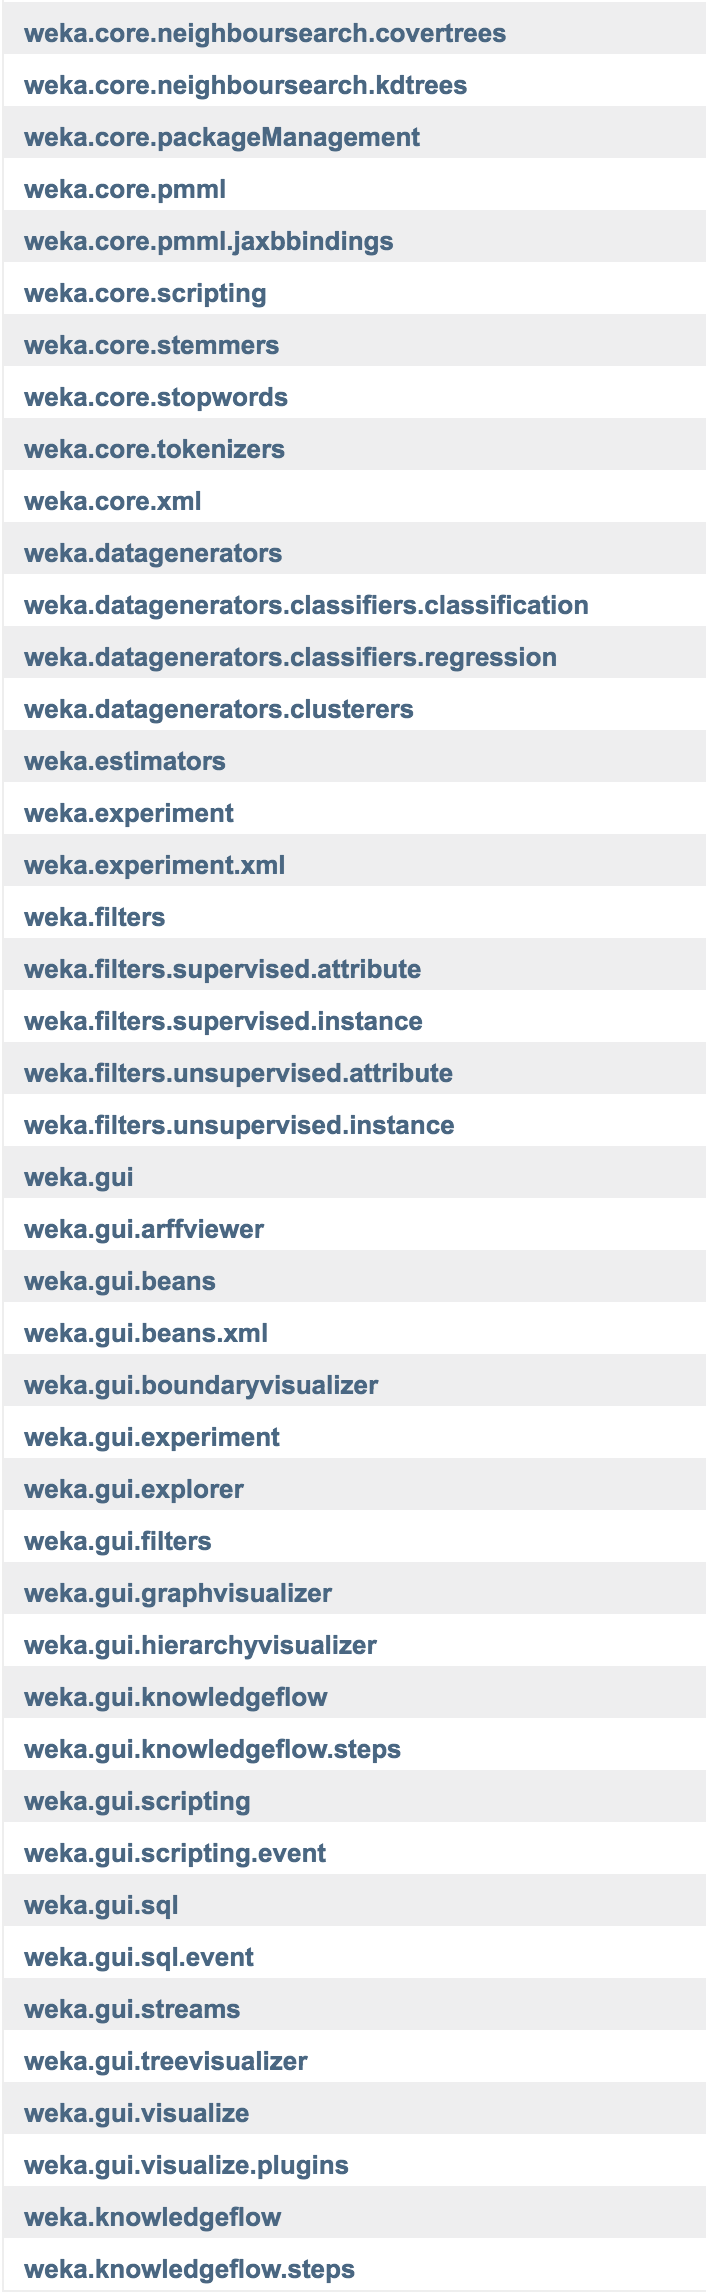
\includegraphics[width=0.45\textwidth]{images/B5_1a2.png}}
\caption{\label{fig:javadoc_a}Javadoc: the front page.}
\end{figure}


When you consult the online documentation generated by Javadoc from
your Web browser, the first thing you see is an alphabetical list of
all the packages in WEKA, as shown in Figure~\ref{fig:javadoc_a}. (If
you view the Javadoc with frames, you will see more than this. Click
on \textit{NO FRAMES} to remove the extra information.) Here we
introduce a few of them in order of importance.

\subsection{The weka.core package}

\begin{figure}[!thp]
\centering
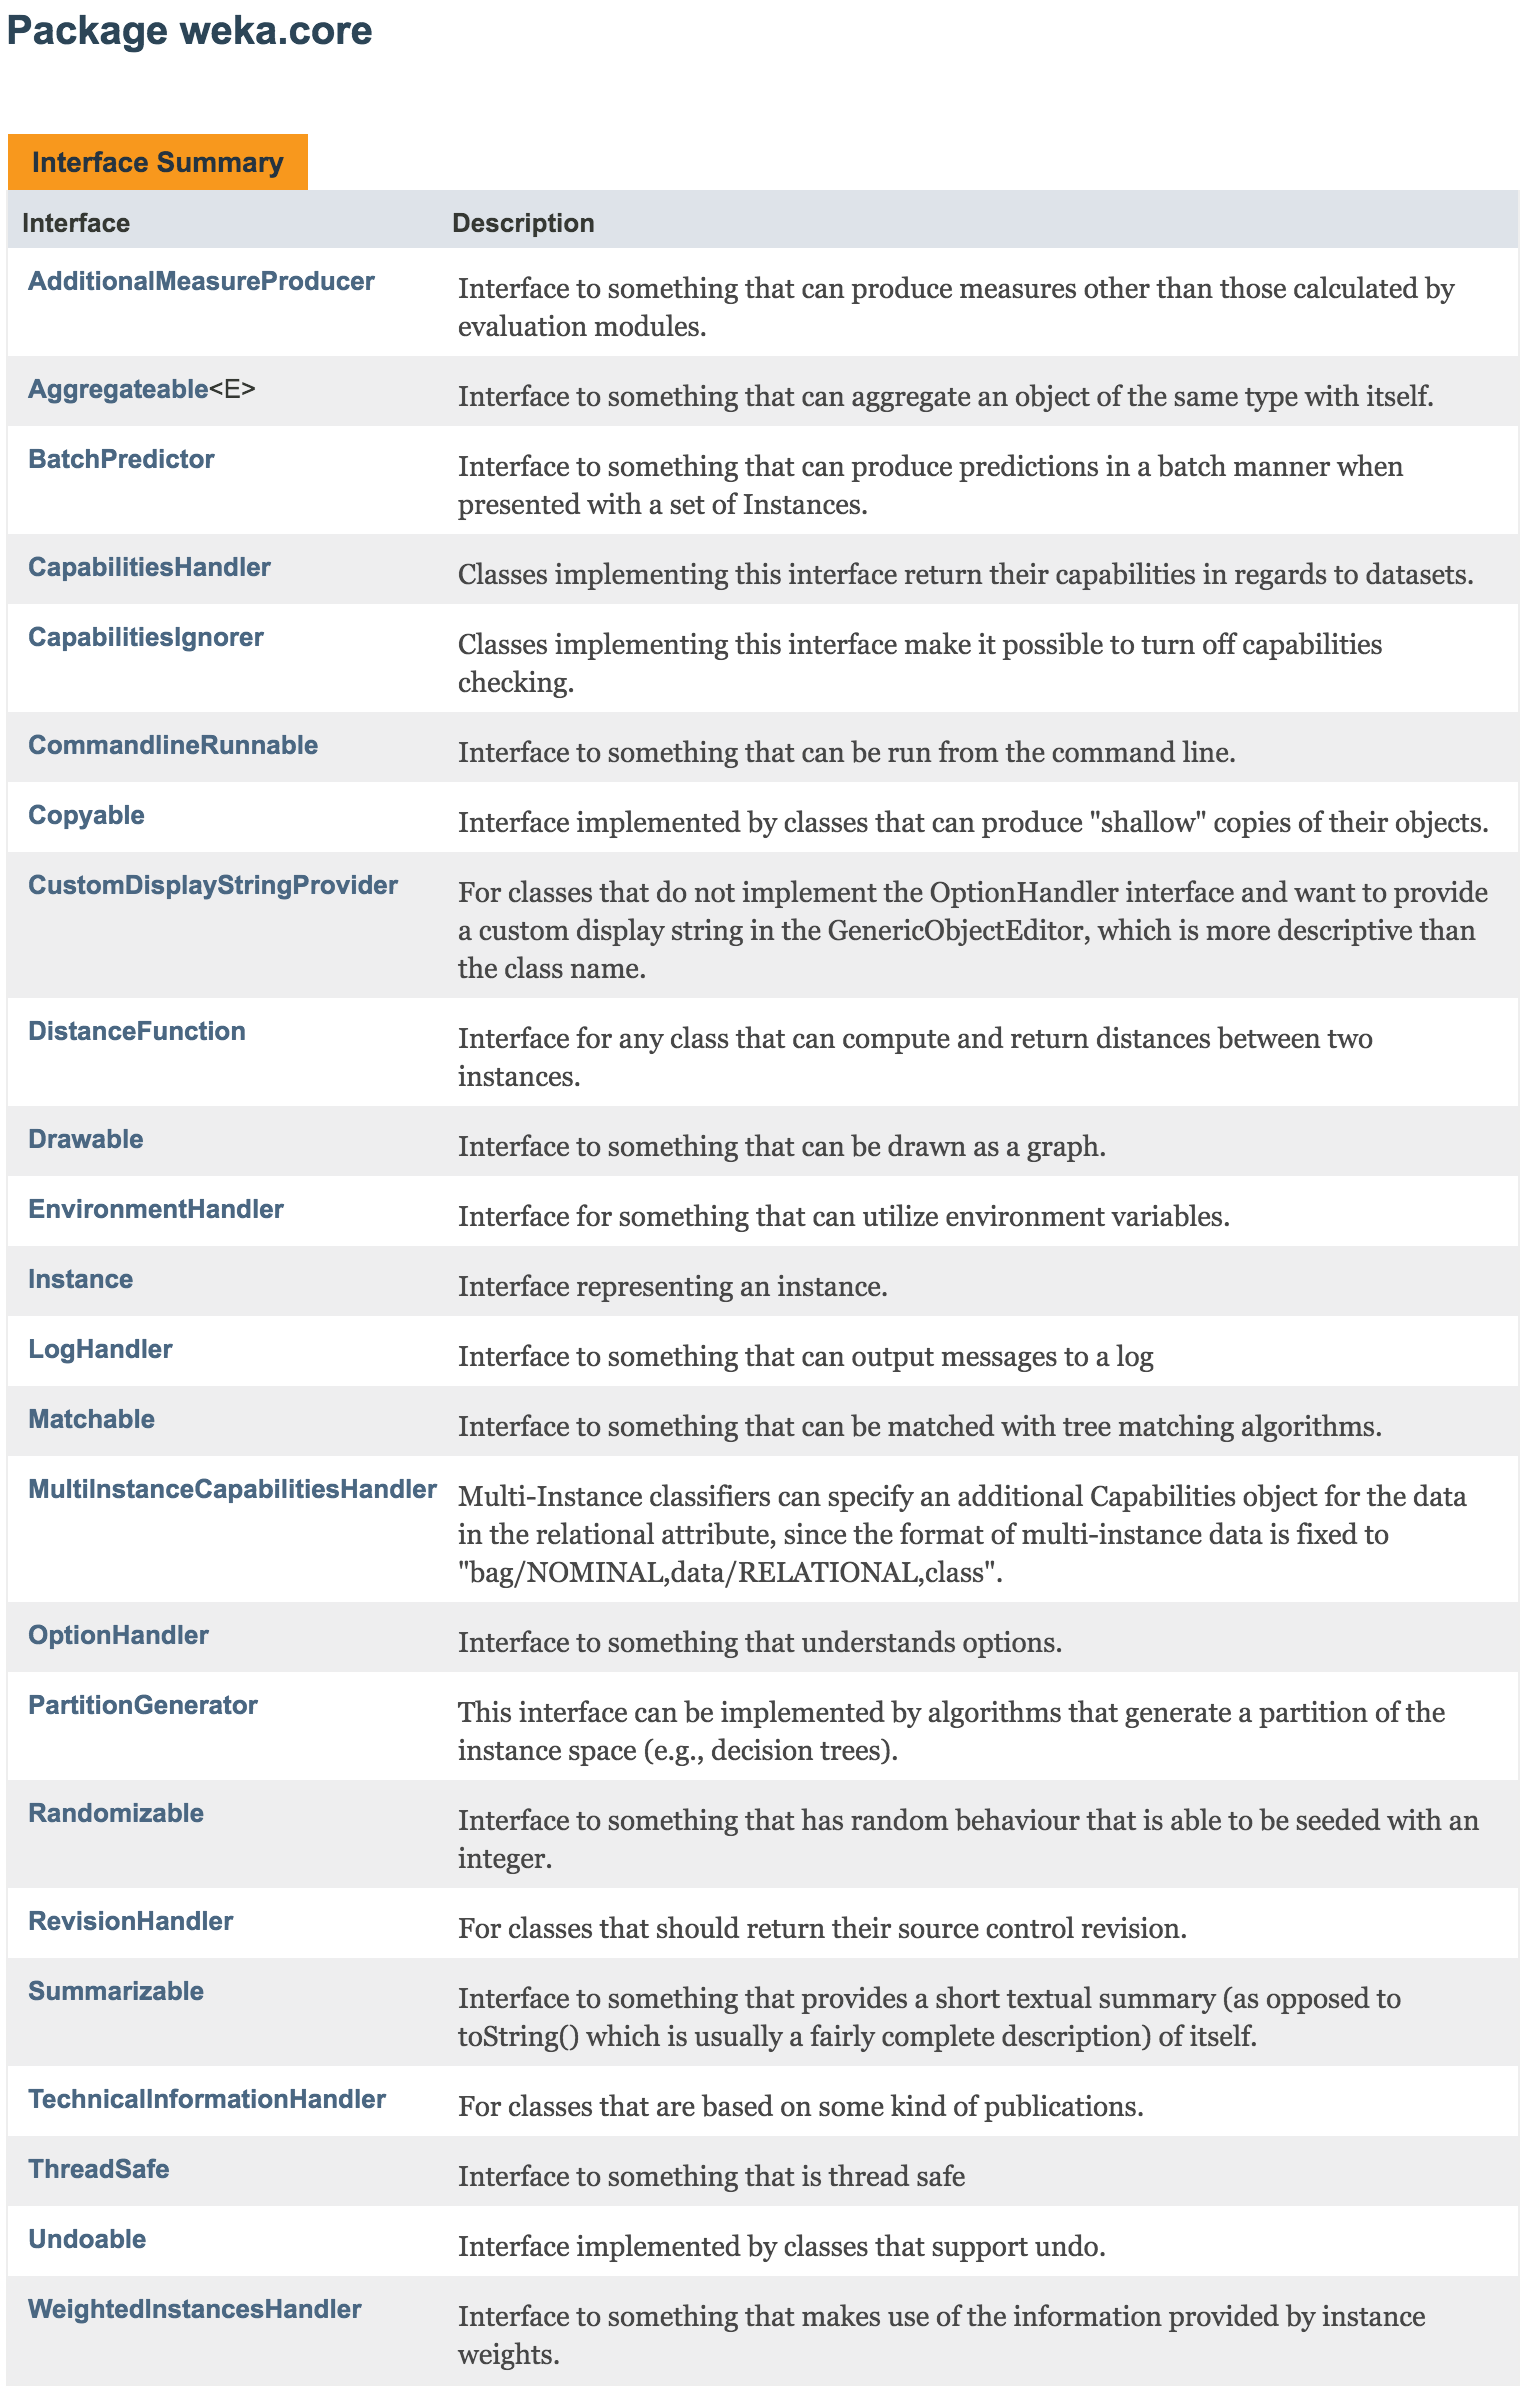
\includegraphics[width=0.9\textwidth]{images/B5_1b1.png}
\label{subfig:javadoc_b_0}
\caption{Javadoc: the \textit{weka.core} package.}
%\phantomcaption
\end{figure}

\begin{figure}[!thp]
\ContinuedFloat
\centering
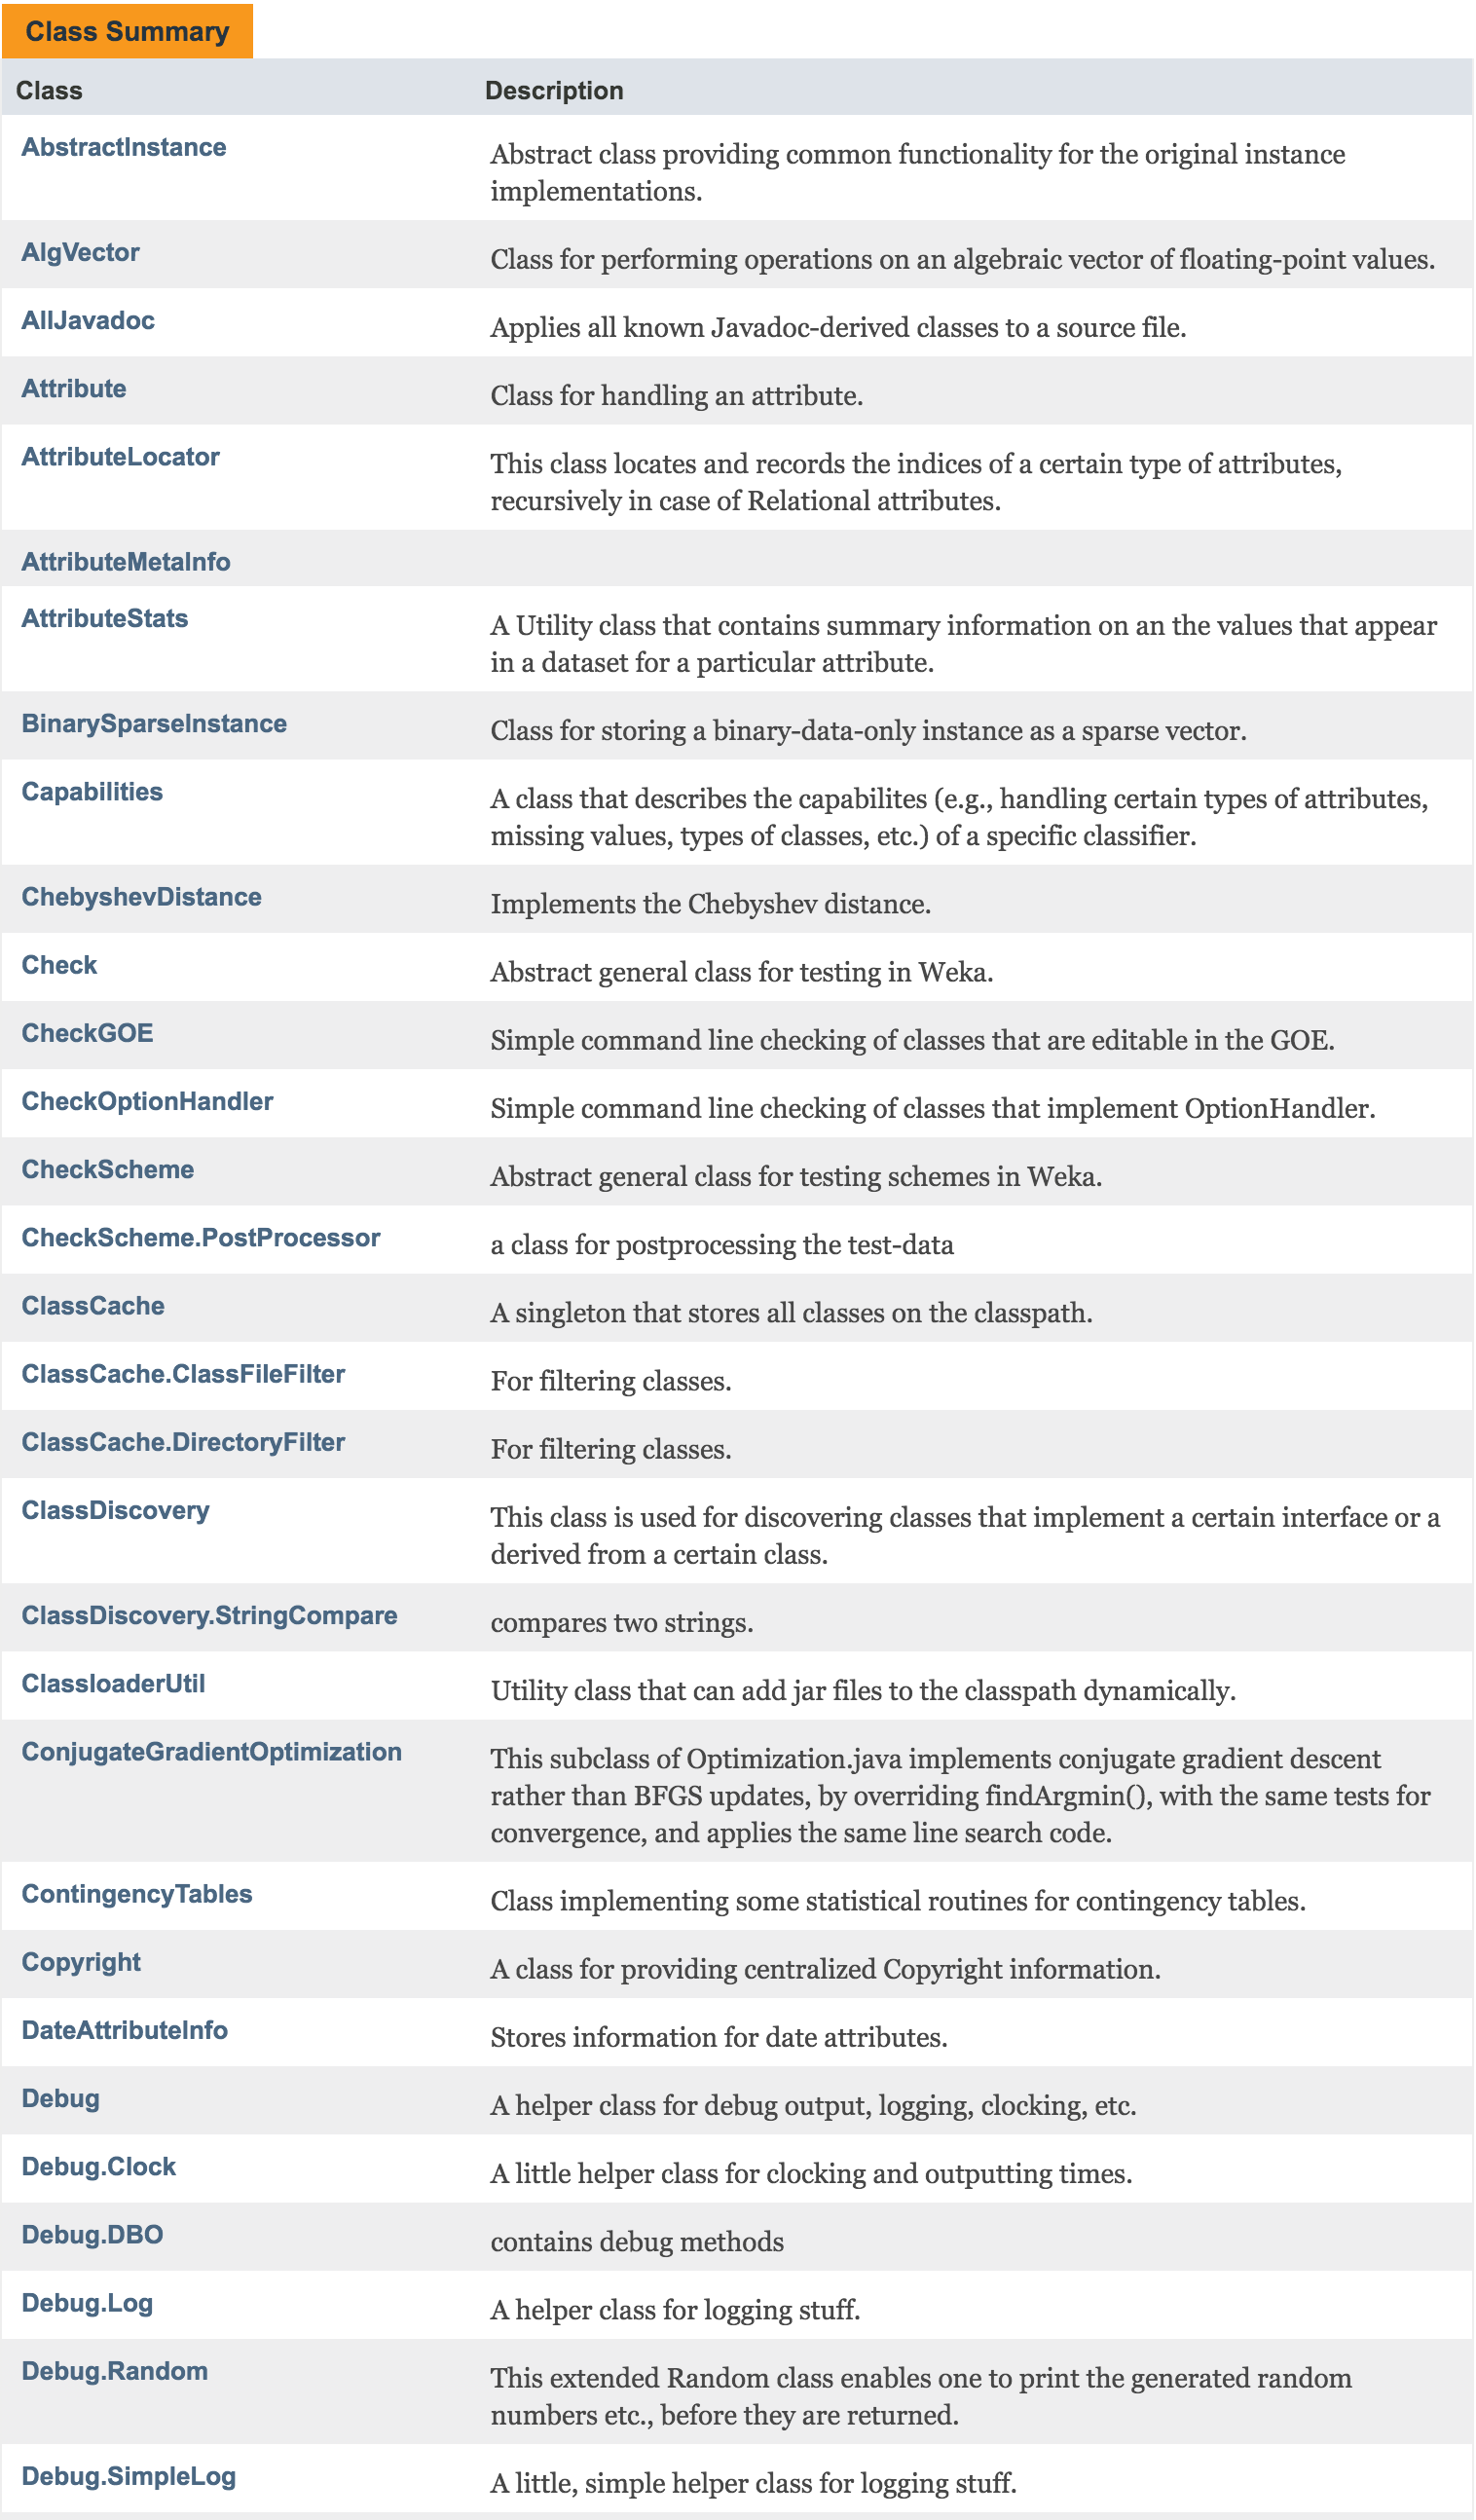
\includegraphics[width=0.9\textwidth]{images/B5_1b2_1.png}
\caption{Javadoc: the \textit{weka.core} package cont.}
%\phantomcaption
\end{figure}

\begin{figure}[!thp]
\ContinuedFloat
\centering
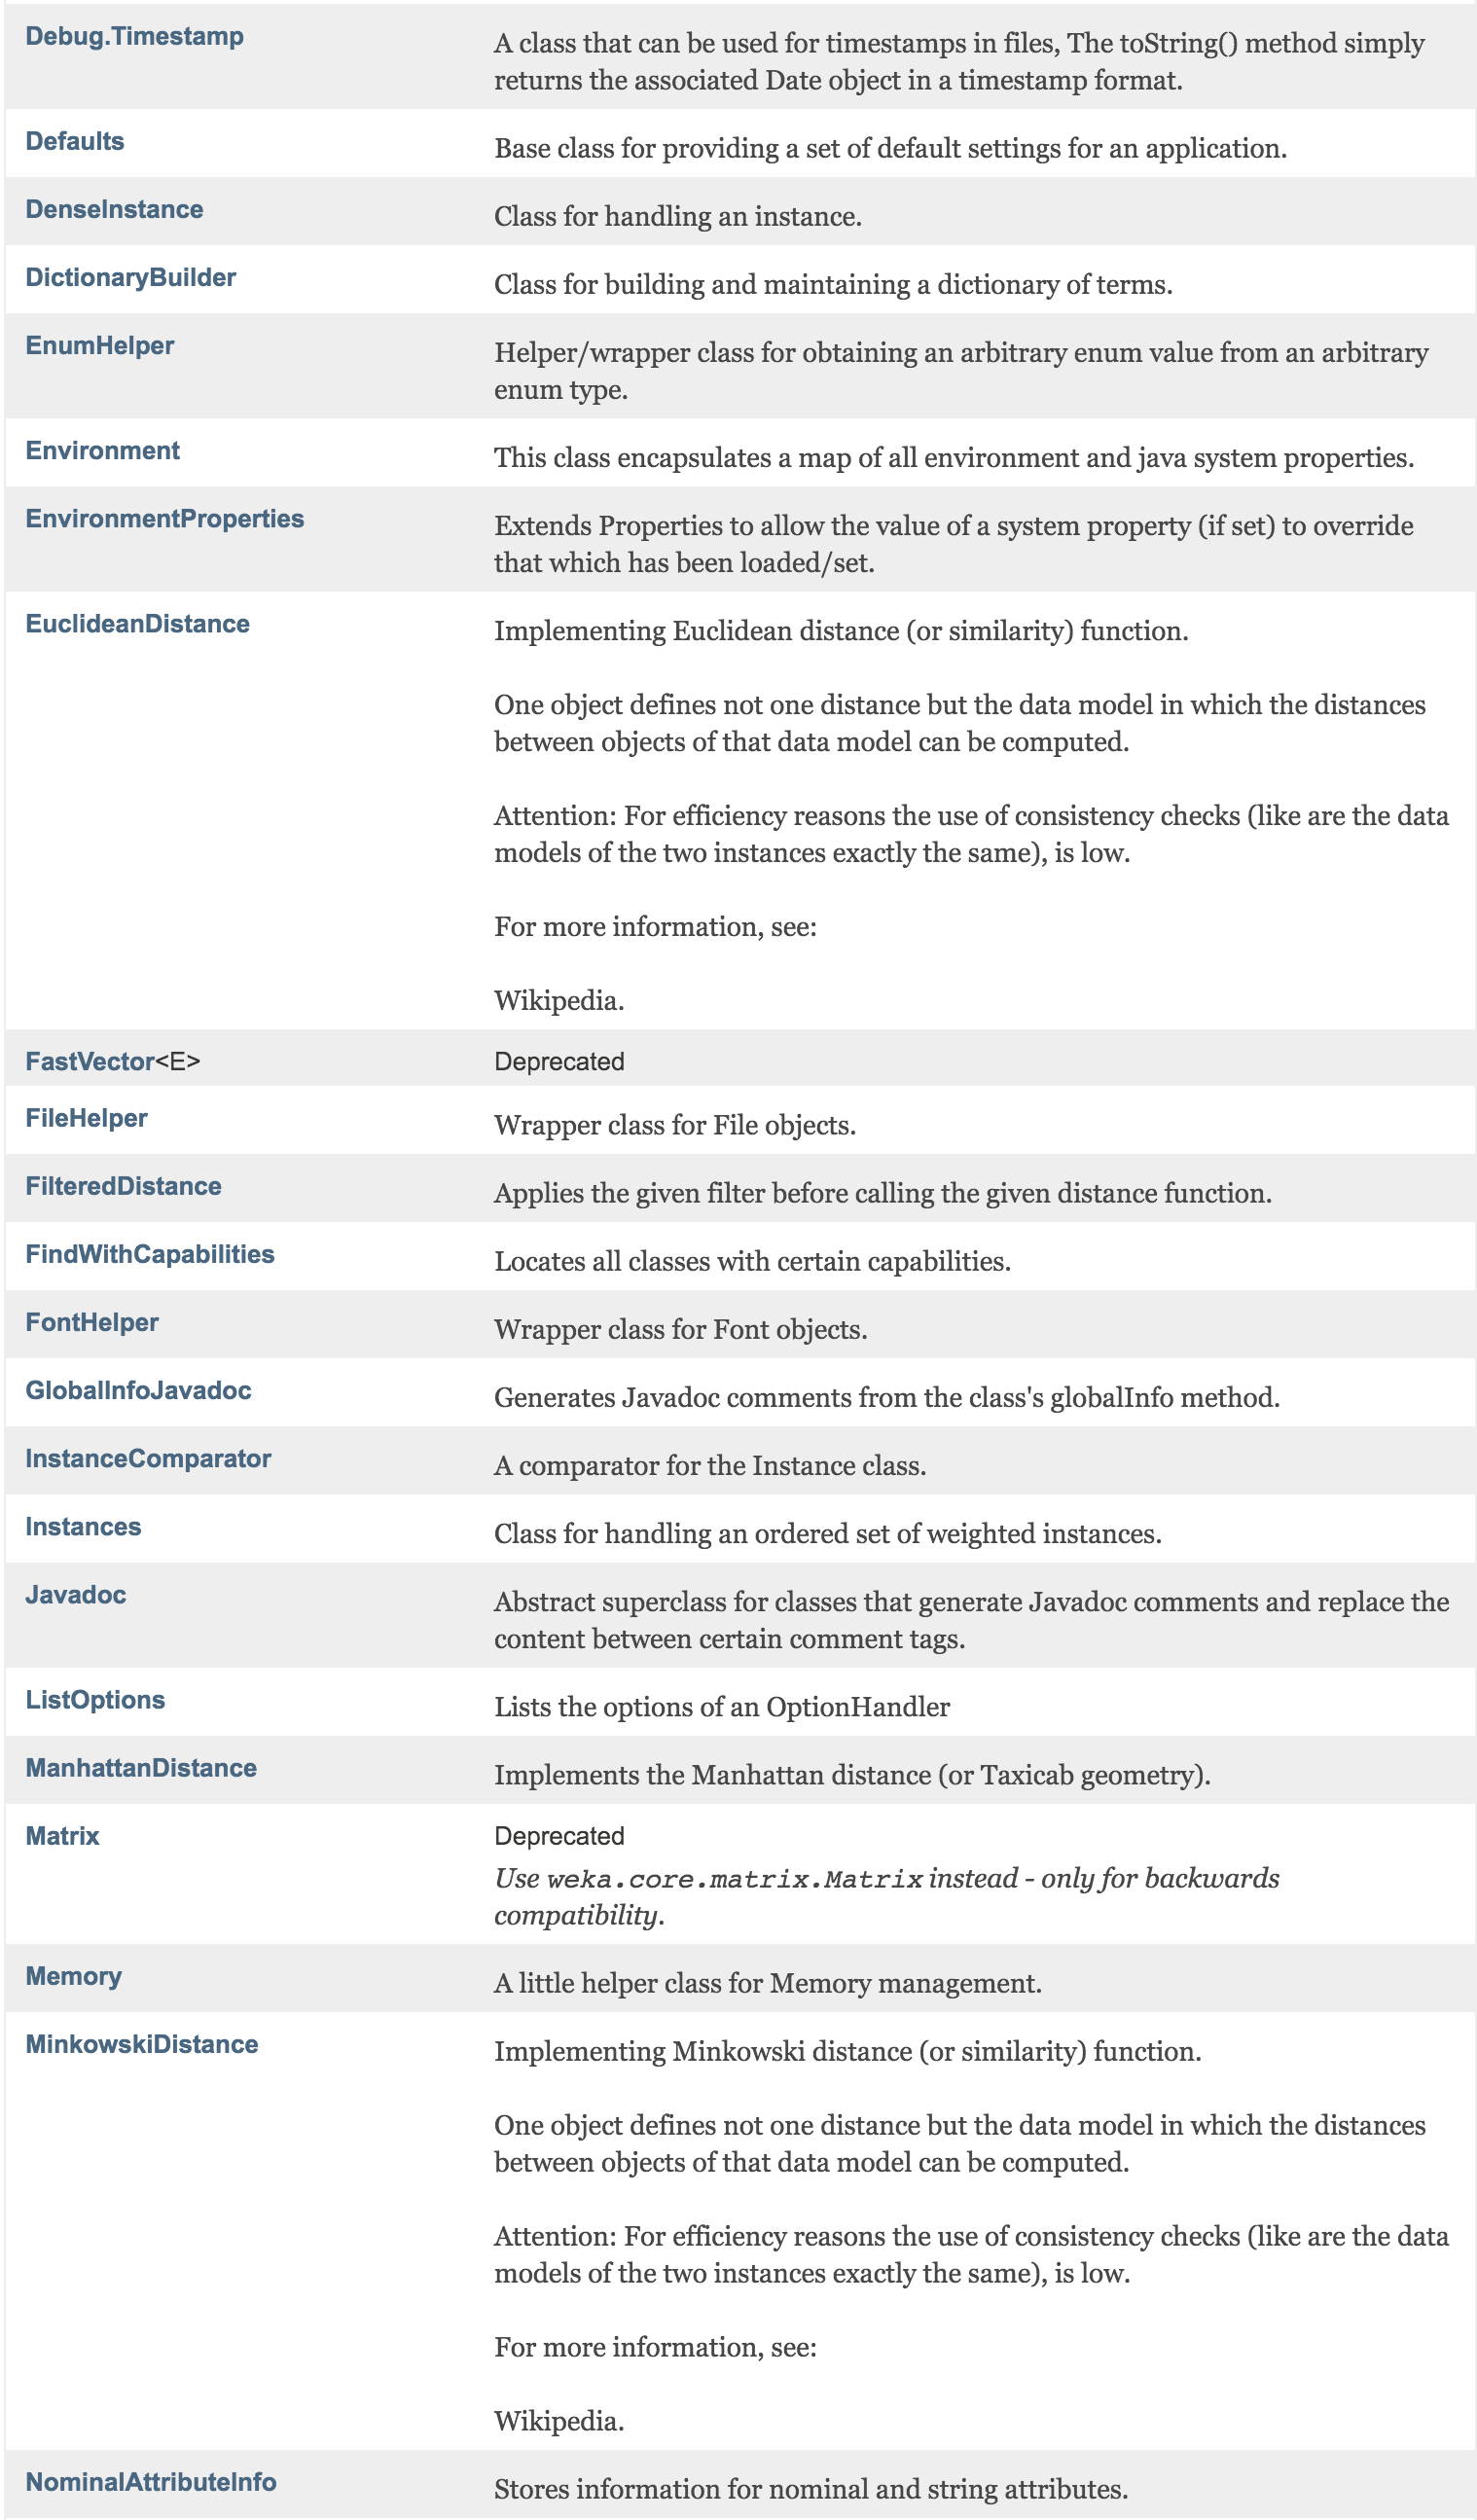
\includegraphics[width=0.95\textwidth]{images/B5_1b2_2.png}
\caption{Javadoc: the \textit{weka.core} package cont.}
%\phantomcaption
\end{figure}

\begin{figure}[!thp]
\ContinuedFloat
\centering
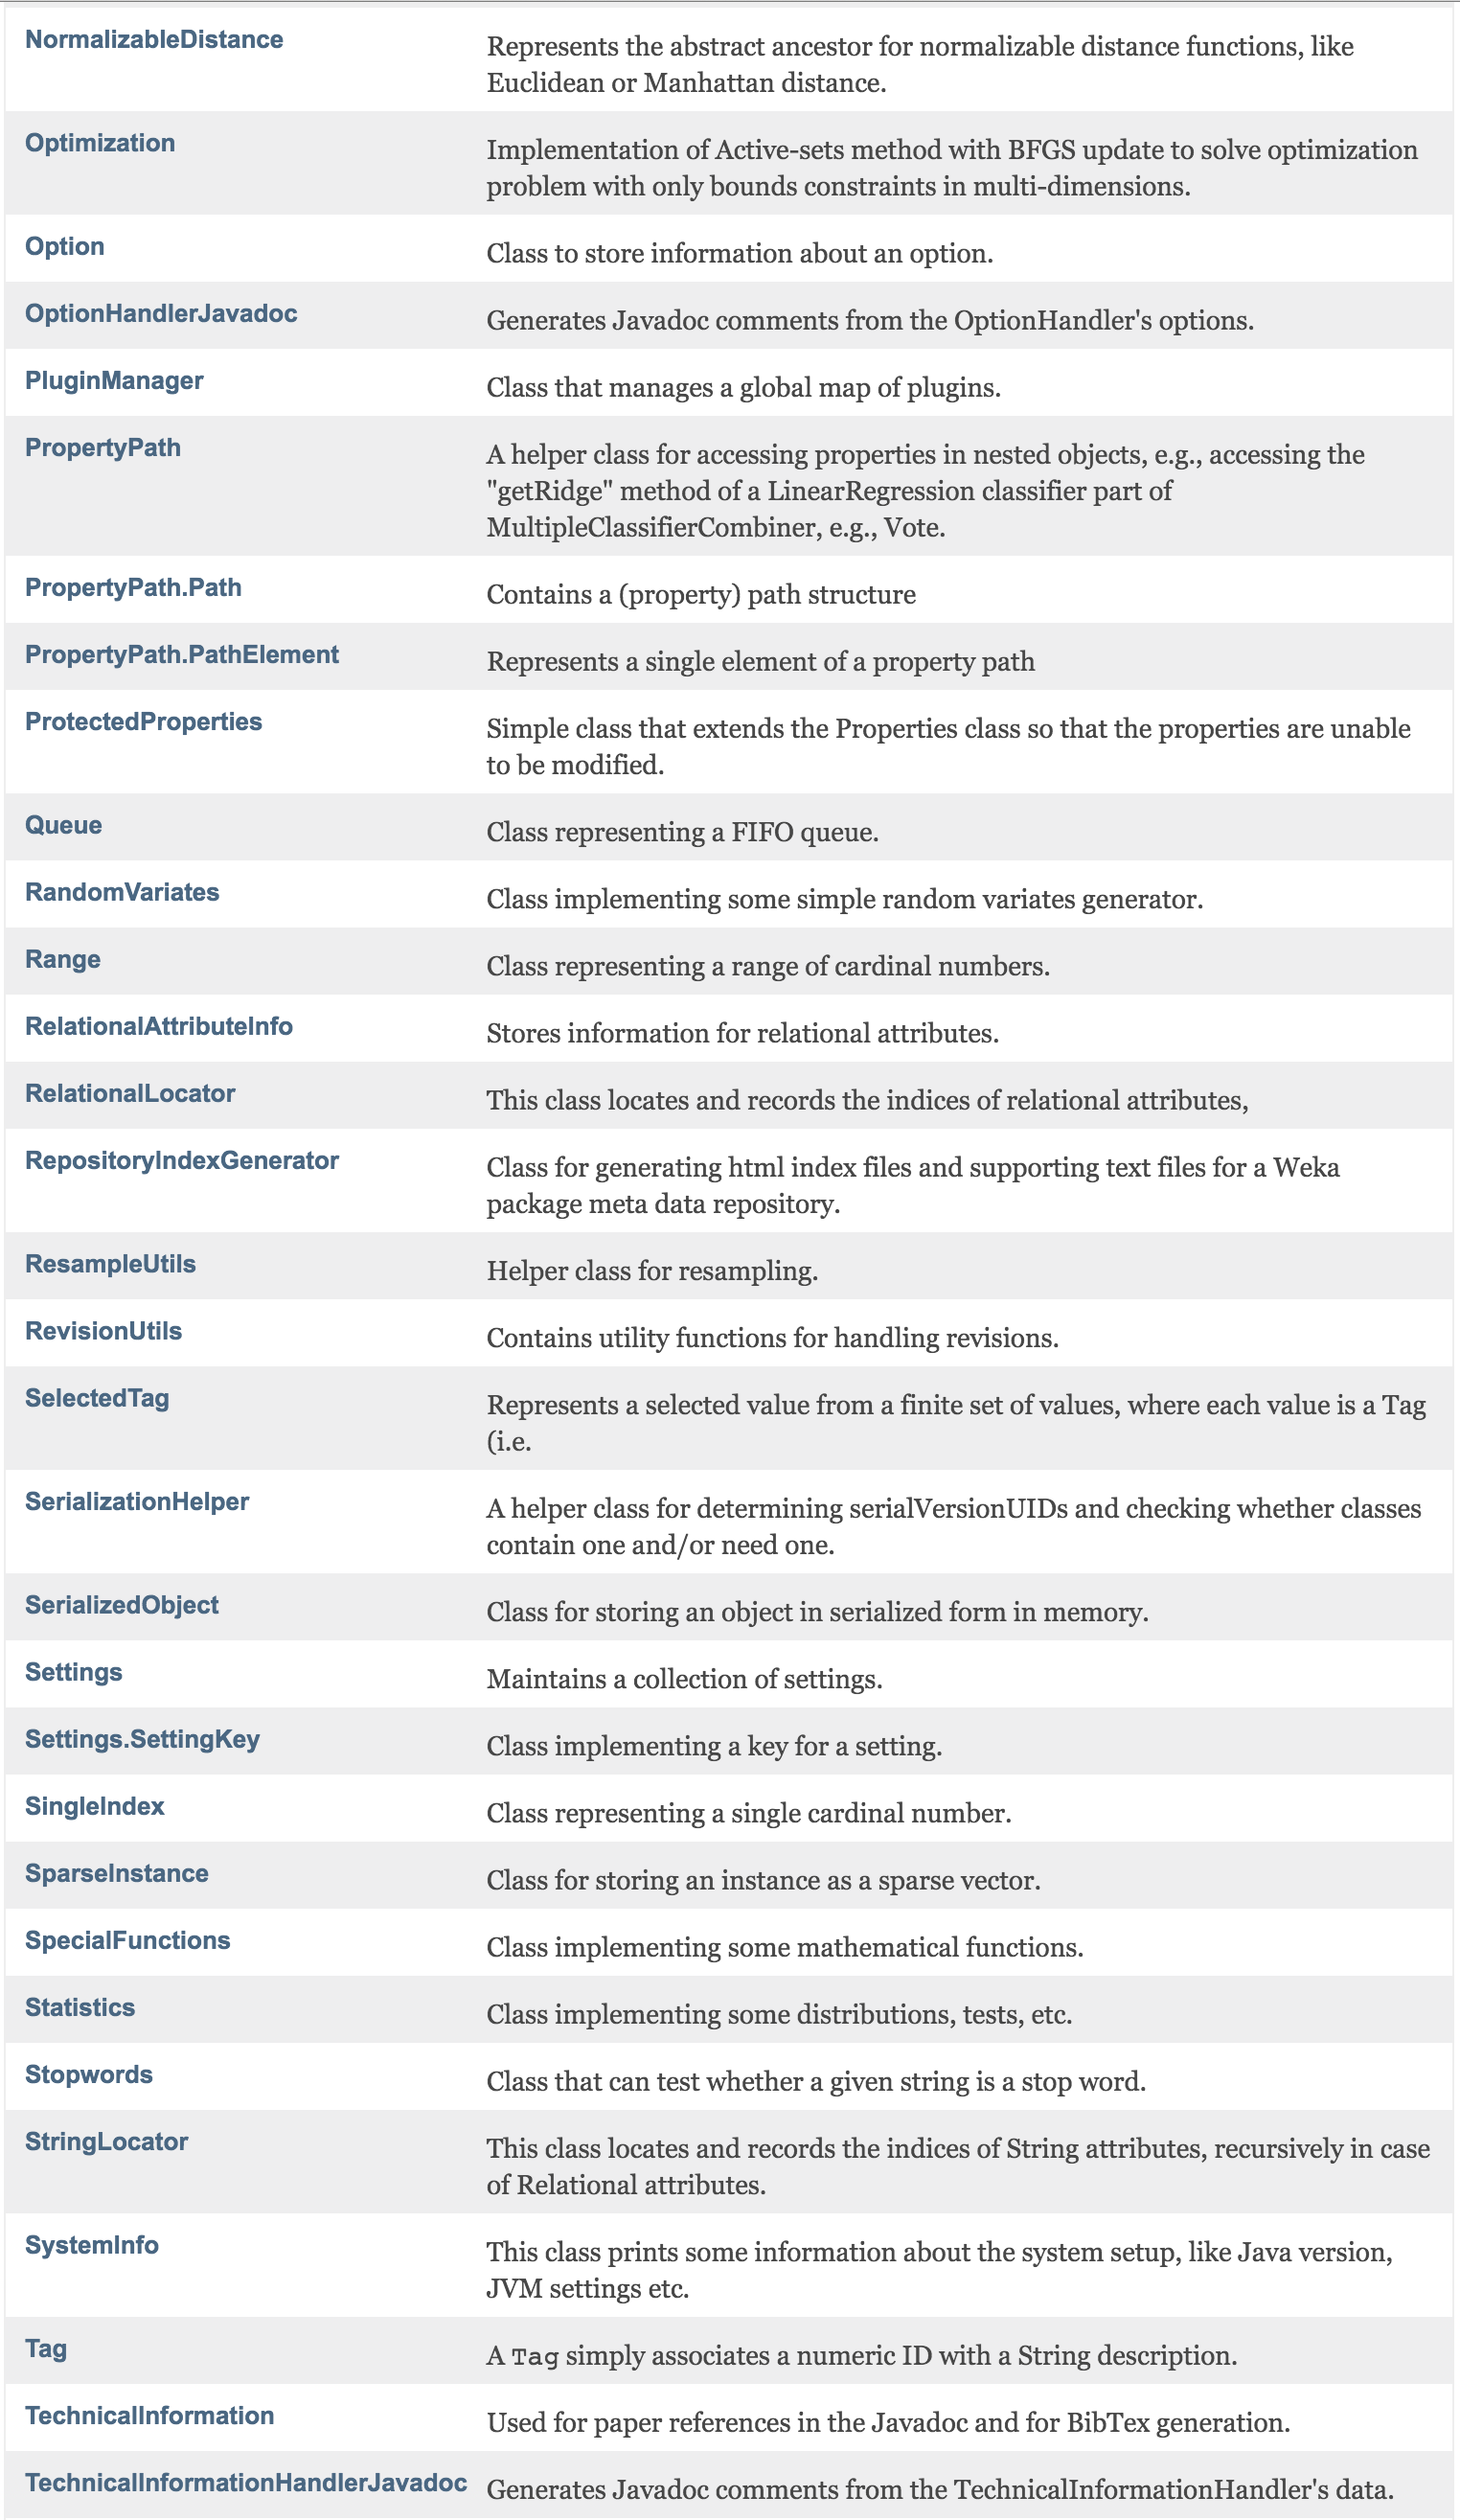
\includegraphics[width=0.95\textwidth]{images/B5_1b2_3.png}
\caption{Javadoc: the \textit{weka.core} package cont.}
%\phantomcaption
\end{figure}

\begin{figure}[!thp]
\ContinuedFloat
\centering
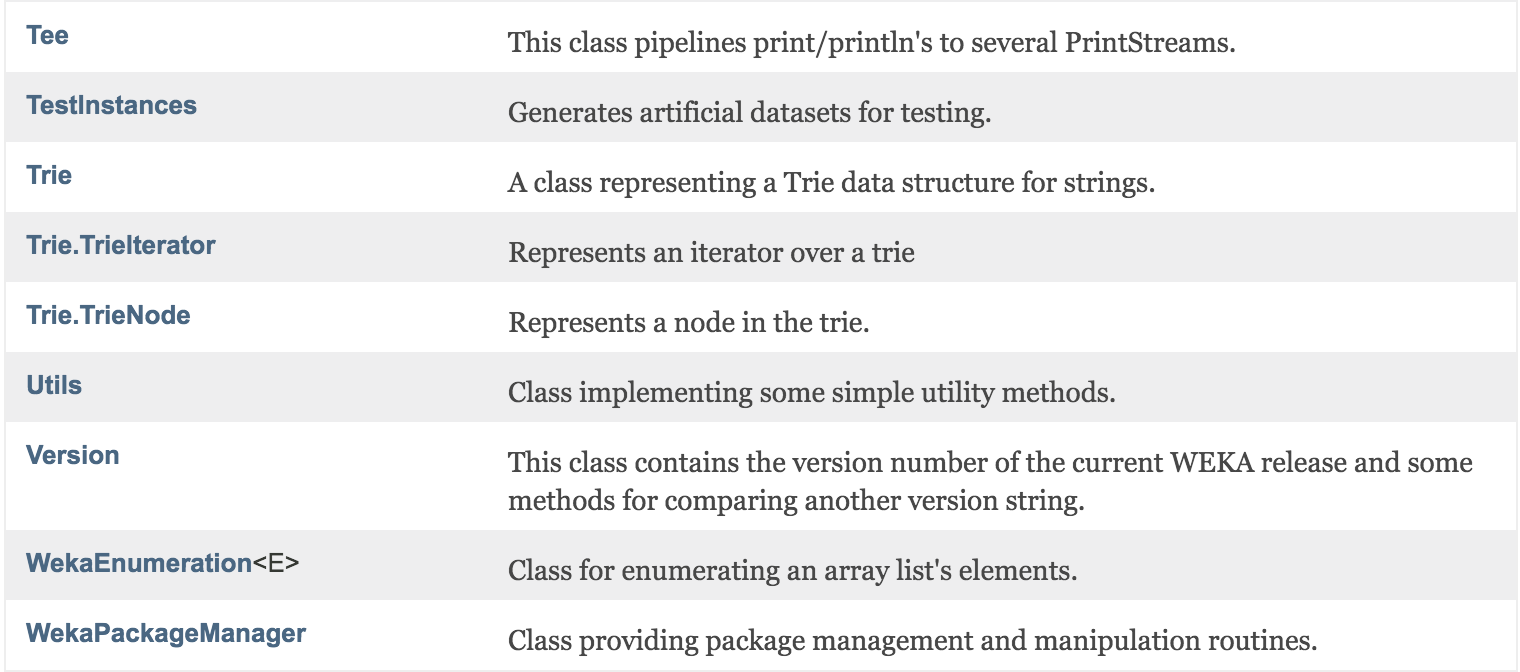
\includegraphics[width=0.95\textwidth]{images/B5_1b2_4.png}
\caption{Javadoc: the \textit{weka.core} package cont.}
\label{fig:javadoc_b}
\end{figure}

The \textit{core} package is central to the WEKA system, and its
classes are accessed from almost every other class. You can determine
what they are by clicking on the \textit{weka.core} hyperlink, which
brings up the Web page shown in Figure~\ref{fig:javadoc_b}.

This Web page is divided into several parts, the main ones being the
\textit{interface summary} and the \textit{class summary}. The latter
is a list of classes contained within the package, and the former
lists the interfaces it provides. An interface is similar to a class,
the only difference being that it doesn't actually do anything by
itself---it is merely a list of methods without actual
implementations. Other classes can declare that they ``implement'' a
particular interface and then provide code for its methods. For
example, the \textit{OptionHandler} interface defines those methods
that are implemented by all classes that can process command-line
options, including all classifiers.

The key classes in the core package are \textit{Attribute},
\textit{Instance}, and \textit{Instances}. An object of class
\textit{Attribute} represents an attribute. It contains the
attribute's name, its type, and, in the case of a nominal or string
attribute, its possible values. An object of class \textit{Instance}
contains the attribute values of a particular instance; and an object
of class \textit{Instances} holds an ordered set of instances, in
other words, a dataset. You can learn more about these classes by
clicking their hyperlinks; we return to them in
Chapter~\ref{chapt:embedded} when we show how to invoke machine
learning schemes from other Java code. However, you can use WEKA from
the command line without knowing the details.

Clicking the \textit{Overview} hyperlink in the upper left corner of
any documentation page returns you to the listing of all the packages
in WEKA that is shown in Figure~\ref{fig:javadoc_a}.

\subsection{The weka.classifiers package}

The \textit{classifiers} package contains implementations of most of
the algorithms for classification and numeric prediction described in
this book. (Numeric prediction is included in \textit{classifiers}: it
is interpreted as prediction of a continuous class.) The most
important class in this package is \textit{AbstractClassifier}, which
implements the \textit{Classifier} interface. \textit{Classifier}
defines the general structure of any scheme for classification or
numeric prediction and declares three important methods,
\textit{buildClassifier()}, \textit{classifyInstance()}, and
\textit{distributionForInstance()}. In the terminology of object-oriented
programming, the learning algorithms are represented by subclasses of
\textit{AbstractClassifier} and therefore automatically inherit these three
methods. Every scheme redefines them according to how it builds a
classifier and how it classifies instances. This gives a uniform
interface for building and using classifiers from other Java
code. Hence, for example, the same evaluation module can be used to
evaluate the performance of any classifier in WEKA.

\begin{figure}[!thp]
\centering
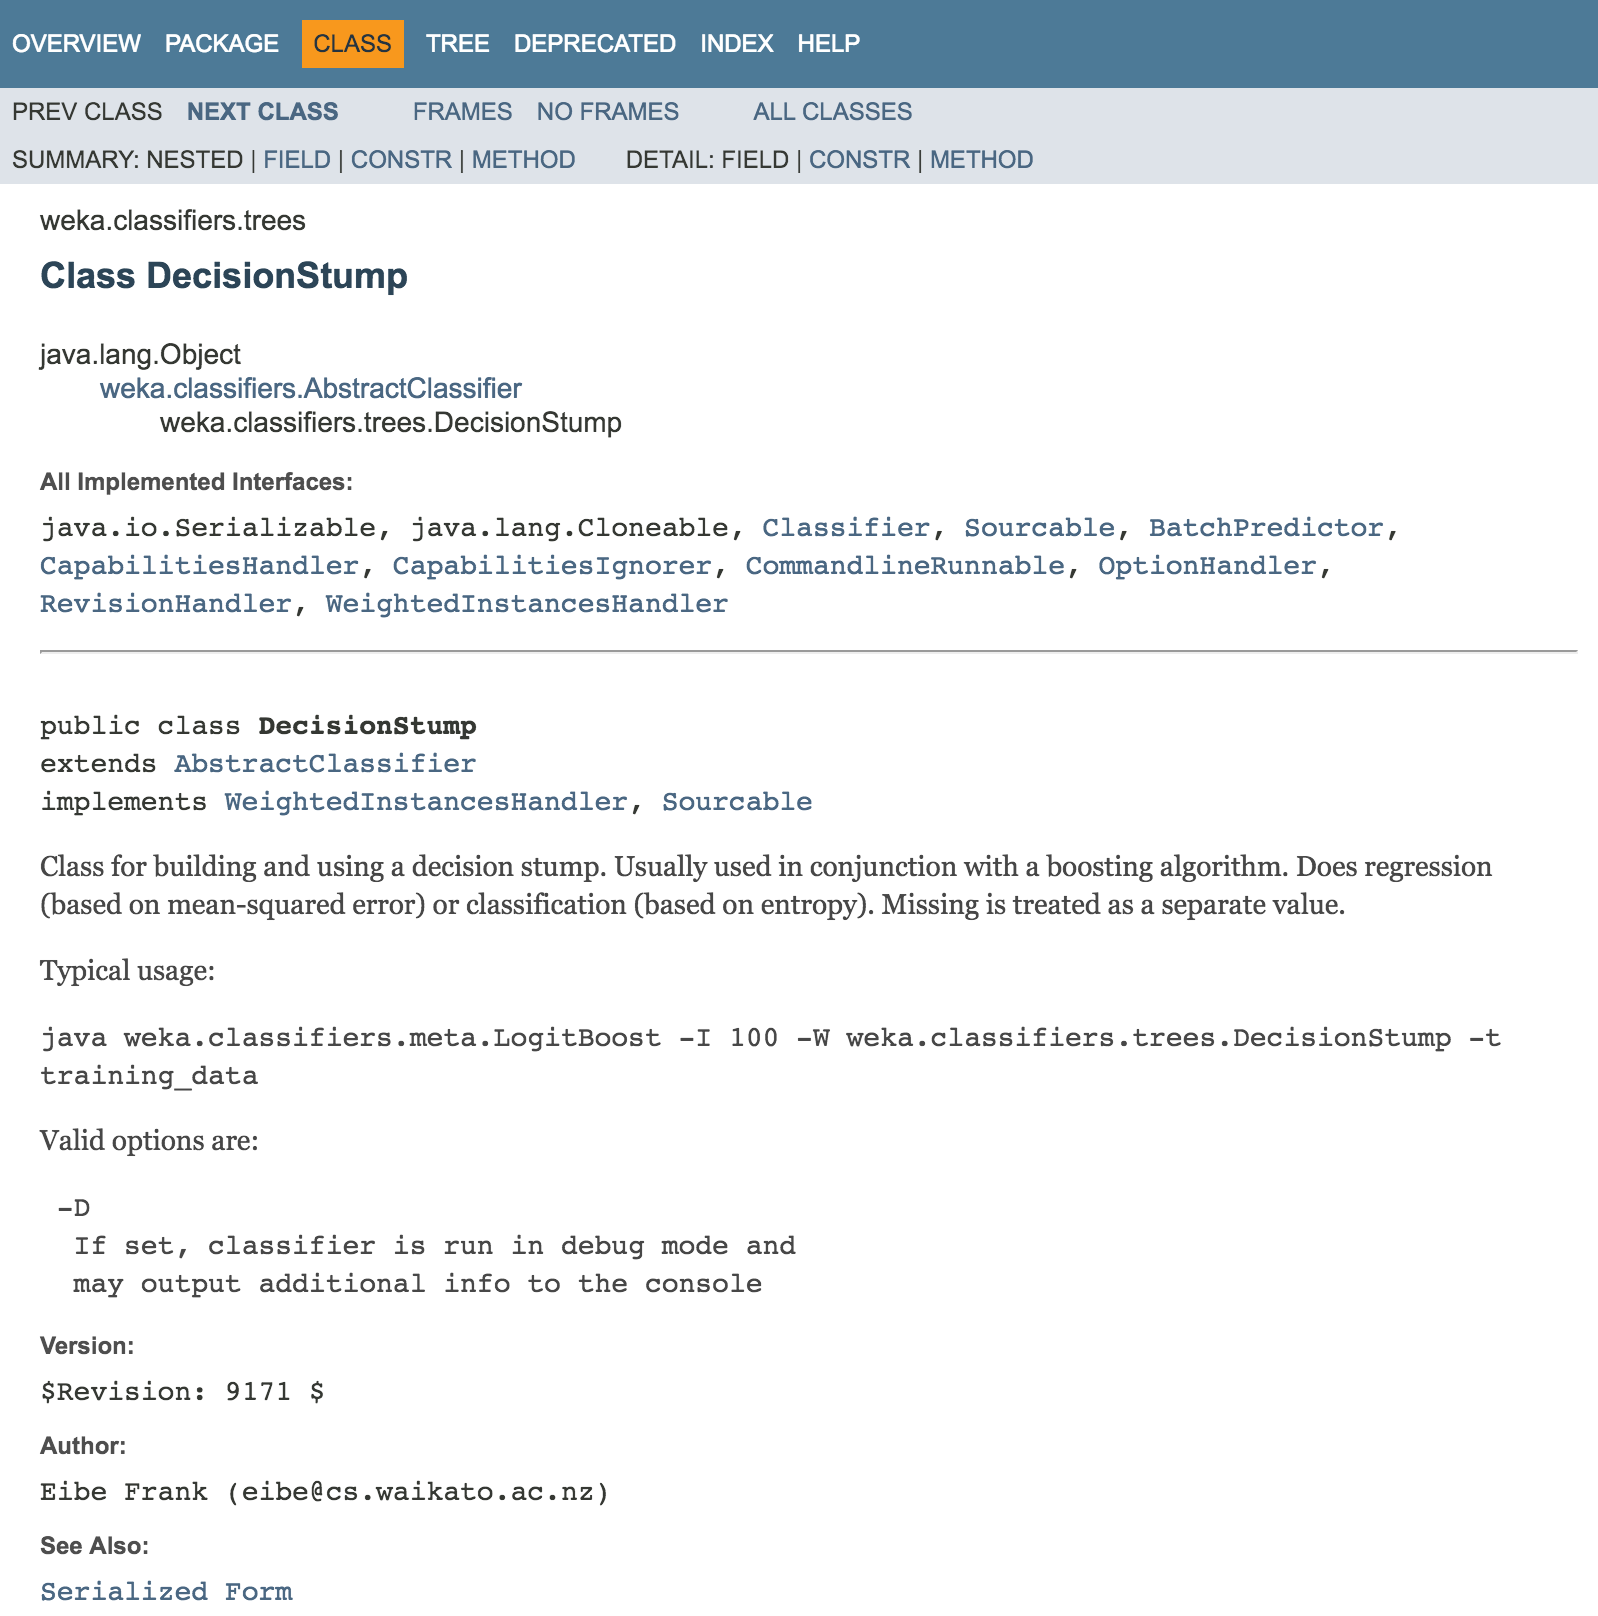
\includegraphics[width=0.9\textwidth]{images/B5_2a.png}
\caption{\textit{DecisionStump}: a class of the \textit{weka.classifiers.trees} package.}
%\phantomcaption
\end{figure}

\begin{figure}[!thp]
\ContinuedFloat
\centering
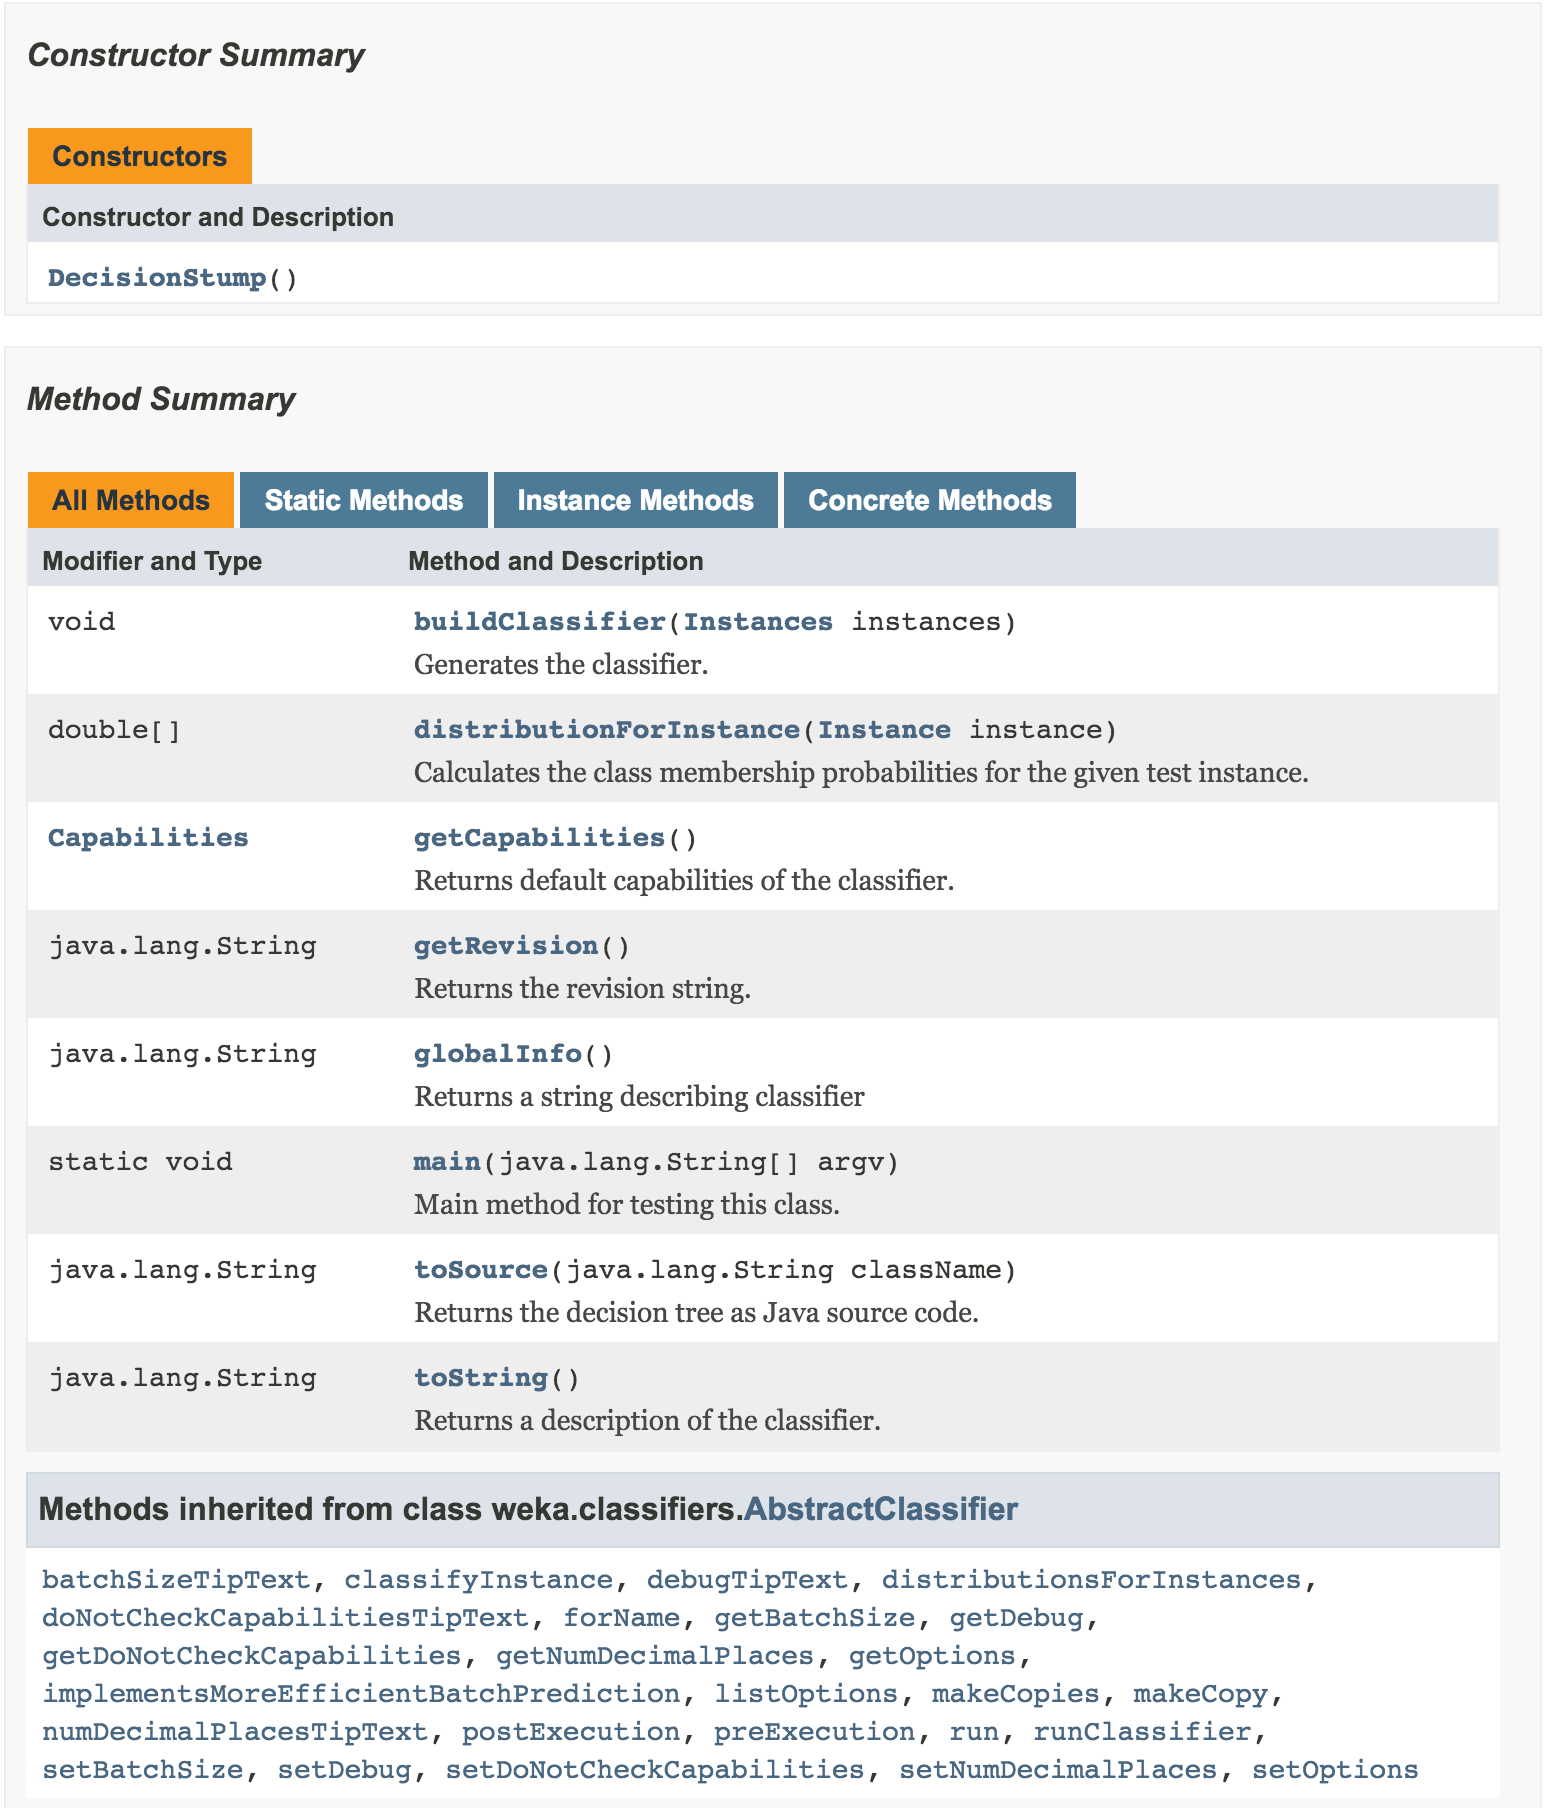
\includegraphics[width=0.9\textwidth]{images/B5_2b.png}
\caption{\textit{DecisionStump}: a class of the \textit{weka.classifiers.trees} package cont.}
\label{fig:javadoc_decisionstump}
\end{figure}

To see an example, click on \textit{weka.classifiers.trees} and then on
\textit{DecisionStump}, which is a class for building a simple one-level binary
decision tree (with an extra branch for missing values). Its
documentation page, shown in Figure~\ref{fig:javadoc_decisionstump},
shows the fully qualified name of this class,
\textit{weka.classifiers.trees.DecisionStump}, near the top. You have to use
this rather lengthy name whenever you build a decision stump from the
command line. The class name is sited in a small tree structure
showing the relevant part of the class hierarchy. As you can see,
\textit{DecisionStump} is a subclass of \textit{weka.classifiers.AbstractClassifier},
which is itself a subclass
of \textit{java.lang.Object}. The \textit{Object} class is the most
general one in Java: all classes are automatically subclasses of it.

After some generic information about the class—brief documentation,
its version, and the author---Figure~\ref{fig:javadoc_decisionstump}
gives an index of the constructors and methods of this class. A
constructor is a special kind of method that is called whenever an
object of that class is created, usually initializing the variables
that collectively define its state. The index of methods lists the
name of each one, the type of parameters it takes, and a short
description of its functionality. Beneath those indexes, the Web page
gives more details about the constructors and methods. We return to
these details later.

As you can see, \textit{DecisionStump} overwrites
the \textit{distributionForInstance()} method
from \textit{AbstractClassifier}: the default implementation
of \textit{classifyInstance()} in \textit{AbstractClassifier} then
uses this method to produce its classifications. In addition, it
contains the \textit{getCapabilities()}, \textit{getRevision()}, \textit{globalInfo()},
\textit{toSource()}, \textit{toString()}, and \textit{main()} methods. We discuss
\textit{getCapabilities()} shortly. The \textit{getRevision()} method simply returns the
revision number of the classifier. There is a utility class in the
\textit{weka.core} package that prints it to the screen, which is used by WEKA
maintainers when diagnosing and debugging problems reported by
users. The \textit{globalInfo()} method returns a string describing the
classifier, which, along with the scheme's options, is displayed by
the \textit{More} button in the generic object editor. The
\textit{toString()} method returns a textual representation of the classifier,
used whenever it is printed on the screen, while
the \textit{toSource()} method is used to obtain a source code
representation of the learned classifier. \textit{The main()} method is called
when you ask for a decision stump from the command line, in other
words, every time you enter a command beginning with

\begin{Verbatim}[fontsize=\footnotesize]
java weka.classifiers.trees.DecisionStump
\end{Verbatim}

\noindent The presence of a \textit{main()} method in a class indicates that it
can be run from the command line: all learning methods and filter
algorithms implement it.

The \textit{getCapabilities()} method is called by the generic object
editor to provide information about the capabilities of a learning
scheme (Figure~\ref{subfig:filters_4}). The training data is checked
against the learning scheme's capabilities when
the \textit{buildClassifier()} method is called, and an error raised
when the classifier's stated capabilities do not match the data's
characteristics. The \textit{getCapabilities()} method is present in
the \textit{AbstractClassifier} class and, by default, enables all
capabilities (i.e., imposes no constraints). This makes it easier for
new WEKA programmers to get started, because they need not learn about
and specify capabilities initially. Capabilities are covered in more
detail in Chapter~\ref{chapt:writing_learning_schemes}.

\subsection{Other packages}

Several other packages listed in Figure~\ref{fig:javadoc_a} are worth mentioning:
\textit{weka.associations}, \textit{weka.clusterers}, \textit{weka.datagenerators},
\textit{weka.estimators}, \textit{weka.filters}, and \newline
\textit{weka.attributeSelection}. The
\textit{weka.associations} package contains association rule learners. These
have been placed in a separate package because association rules are
fundamentally different from classifiers. The \textit{weka.clusterers} package
contains methods for unsupervised learning. Artificial data can be
generated using the classes in \textit{weka.datagenerators}. The
\textit{weka.estimators} package contains subclasses of a generic \textit{Estimator}
class, which computes different types of probability
distributions. These subclasses are used by the Naive Bayes algorithm
(among others).

In the \textit{weka.filters package}, the \textit{Filter} class
defines the general structure of classes containing filter algorithms,
which are all implemented as subclasses of \textit{Filter}. Like classifiers,
filters can be used from the command line: we will see how
shortly. The \textit{weka.attributeSelection} package contains several classes
for attribute selection. These are used by the
\textit{AttributeSelectionFilter} in \newline
\textit{weka.filters.supervised.attribute}, but can also be invoked separately.

\subsection{Javadoc indexes}

As mentioned previously, all classes are automatically subclasses of
\textit{Object}. To examine the tree that corresponds to WEKA's hierarchy of
classes, select the \textit{Overview} link from the top of any page of
the online documentation. Click Tree to display the overview as a tree
that shows which classes are subclasses or superclasses of a
particular class---for example, which classes inherit from
\textit{AbstractClassifier}.

The online documentation contains an index of all classes, packages,
publicly accessible variables (called \textit{fields}) and methods in
WEKA---in other words, all fields and methods that you can access from
your own Java code. To view it, click \textit{Overview} and
then \textit{Index}.

Suppose you want to check which WEKA classifiers and filters are
capable of operating incrementally. Searching for the word \textit{incremental}
in the index would soon lead you to the keyword
\textit{UpdateableClassifier}. In fact, this is a Java interface; interfaces
are listed after the classes in the overview tree. You are looking for
all classes that implement this interface. Clicking any occurrence of
it in the documentation brings up a page that describes the interface
and lists the classifiers that implement it. To find the filters is a
little trickier unless you know the keyword \textit{StreamableFilter}, which is
the name of the interface that streams data through a filter: again
its page lists the filters that implement it. You would stumble across
that keyword if you knew any example of a filter that could operate
incrementally.

\section{Command-line options}
\label{section:command_line_opts}

In the preceding example, the \textit{--t} option was used on the
command line to communicate the name of the training file to the
learning algorithm. There are many other options that can be used with
any learning scheme, and also scheme-specific ones that apply only to
particular schemes. If you invoke a scheme with the \textit{--h}
or \textit{--help} option, or without any command-line options at all,
it displays the applicable options: first the general options, then
the scheme-specific ones. In the command-line interface, type:

\begin{Verbatim}[fontsize=\footnotesize]
java weka.Run .J48 -h
\end{Verbatim}

\noindent You'll see a list of the options common to all learning schemes, 
shown in Table~\ref{table:general_command_line_opts}, followed by
those that apply only to \textit{J48}, shown in
Table~\ref{table:j48_command_line_opts}. A notable one
is \textit{--info}, which outputs a very brief description of the
scheme. We will explain the generic options and then briefly review
the scheme-specific ones.

\begin{table}[!thp]
\footnotesize
{\centering \begin{tabular}{ll}
\hline
Option & Function \\
\hline
--h or --help & Print help information \\
--synopsis or --info & In combination with --h or --help, prints \\
& the information from the ``More'' button \\
& in a classifier's generic object editor \\
--t $<$training file$>$ & Specify training file \\
--T $<$test file$>$ & Specify test file. If none, a cross-validation \\
& is performed on the training data \\
--c $<$class index$>$ & Specify index of class attribute \\
--x $<$number of folds$>$ & Specify number of folds for cross-validation \\
--s $<$random number seed$>$ & Specify random number seed for cross-validation \\
--no-cv & Don't perform cross-validation \\
--split-percentage $<$training percentage$>$ & Specify percentage of the data to use for \\
& the training set in a train-test split \\
--preserve-order & Preserve original order of the data when \\ 
& performing a train-test split \\
--m $<$cost matrix file$>$ & Specify file containing cost matrix \\
--l $<$input file$>$ & Specify input file for model \\
--d $<$output file$>$ & Specify output file for model \\
--v & Output no statistics for training data \\
--o & Output statistics only, not the classifier \\ 
--k & Output information-theoretic statistics \\
--p $<$attribute range$>$ & Output predictions for test instances \\
--distribution & In combination with --p, output the full probability \\ 
& distribution for discrete class data \\
& instead of just the predicted label \\
--r & Output cumulative margin distribution \\
--z $<$class name$>$ &Output the source representation of the classifier \\
--g & Output the graph representation of the classifier \\
--xml $<$filename$>$ $|$ $<$xml string$>$ & Set scheme-specific options \\
& from XML encoded options stored in a file or \\ 
& in a supplied string \\
--threshold-file $<$file$>$ & Save threshold data (for ROC curves, etc.) to a file \\
--threshold-label $<$label$>$ & Class label for the threshold data \\
--no-predictions & Turns off the collection of predictions in \\
& order to conserve memory \\
--force-batch-training & Always train classifier in batch mode, \\
& never incrementally \\
--toggle & Comma-separated list of metric names to toggle in \\
&  the outputUses the specified class for \\ 
& generating the classification output \\
--classifications & Uses the specified class for generating the \\
& classification output \\
--do-not-output-per-class-statistics & Suppress the output of \\
& information retrieval statistics for each class \\
\hline
\end{tabular} \footnotesize \par}
\caption{\label{table:general_command_line_opts}Generic options for learning schemes in WEKA}
\end{table}

\begin{table}[thp]
\footnotesize
{\centering \begin{tabular}{ll}
\hline
Option & Function \\
\hline
--U & Use unpruned tree \\
--O & Do not collapse tree \\
--C $<$pruning confidence$>$ & Specify confidence threshold for pruning \\
--M $<$number of instances$>$ & Specify minimum number of instances in \\
& any leaf \\
--R & Use reduced-error pruning \\
--N $<$number of folds$>$ & Specify number of folds for reduced-error \\
& pruning; one fold is used as pruning set \\
--B & Use binary splits only \\
--S & Don't perform subtree raising \\
--L & Retain instance information \\
--A & Smooth the probability estimates using Laplace smoothing \\
--J & Prevent the use of MDL correction for information gain \\
& on numeric attributes \\
--Q & Seed for shuffling the data \\
\hline
\end{tabular} \footnotesize \par}
\caption{\label{table:j48_command_line_opts}Scheme-specific options}
\end{table}

\subsection{Generic options}

The options in Table~\ref{table:general_command_line_opts} determine which
data is used for training and testing, how the classifier is
evaluated, and what kind of statistics are displayed. For example, the
\textit{--T} option is used to provide the name of the test file when evaluating
a learning scheme on an independent test set. By default the class is
the last attribute in an ARFF file, but you can declare another one to
be the class using \textit{--c} followed by the position of the
desired attribute, 1 for the first, 2 for the second, and so on.

When cross-validation is performed (the default if a test file is not
provided), the data is randomly shuffled first. To repeat the
cross-validation several times, each time reshuffling the data in a
different way, set the random number seed with \textit{--s} (default
value 1). With a large dataset you may want to reduce the number of
folds for the cross-validation from the default value of 10
using \textit{--x}. If performance on the training data alone is
required, \textit{--no-cv} can be used to suppress
cross-validation; \textit{--v} suppresses output of performance on the
training data. As an alternative to cross-validation, a train-test
split of the data specified with the \textit{--t} option can be
performed by supplying a percentage to use as the new training set
with \textit{--split-percentage} (the remaining data is used as the test
set). Randomization of the data can be suppressed when performing a
train-test split by specifying \textit{--preserve-order.}

In the Explorer, cost-sensitive evaluation is invoked as described in
Section~\ref{subsec:doing_it_again}. To achieve the same effect from
the command line, use the \textit{--m} option to provide the name of a
file containing the cost matrix. Here is a cost matrix for the weather
data: \newline

\begin{Verbatim}[fontsize=\footnotesize]
2  2   % Number of rows and columns in the matrix
0 10   % If true class yes and prediction no, penalty is 10.
1  0   % If true class no and prediction yes, penalty is 1.
\end{Verbatim}

\noindent The first line gives the number of rows and columns, that is, 
the number of class values. Then comes the matrix of
penalties. Comments introduced by \% can be appended to the end of any
line.

It is also possible to save and load models. If you provide the name
of an output file using \textit{--d}, WEKA saves the classifier
generated from the training data. To evaluate the same classifier on a
new batch of test data, you load it back using \textit{--l} instead of
rebuilding it. If the classifier can be updated incrementally, you can
provide both a training file and an input file, and WEKA will load the
classifier and update it with the given training instances.

If you wish only to assess the performance of a learning scheme, use
\textit{--o} to suppress output of the model. Use \textit{--k} to compute
information-theoretic measures from the probabilities derived by a
learning scheme.

People often want to know which class values the learning scheme
actually predicts for each test instance. The \textit{--p} option
prints each test instance's number, the index of its class value and
the actual value, the index of the predicted class value and the
predicted value, a ``+'' if the class was misclassified, and the
probability of the predicted class value. The probability predicted
for each of the possible class labels of an instance can be output by
using the \textit{--distribution} flag in conjunction
with \textit{--p}. In this case, ``*'' is placed beside the
probability in the distribution that corresponds to the predicted
class value. The \textit{--p} options also outputs attribute values
for each instance and must be followed by a specification of the range
(e.g., 1--2)---use 0 if you don't want any attribute values. You can
also output the cumulative margin distribution for the training data,
which shows the distribution of the margin measure. Finally, you can
output the classifier's source representation, and a graphical
representation if the classifier can produce one.

Data relating to performance graphs such as ROC and recall-precision
curves can be sent to a file using the \textit{--threshold-file}
option. The class label to treat as the positive class for generating
the data can be specified with \textit{--threshold-label}. The next
section discusses how scheme-specific options are supplied on the
command line; they can also be set from an XML file or string using
the \textit{--xml} option.

\begin{table}[!thp]
\footnotesize
{\centering \begin{tabular}{ll}
\hline
Option & Function \\
\hline
--U & Use unpruned tree \\
--O & Do not collapse tree \\
--C $<$pruning confidence$>$ & Specify confidence threshold for pruning \\
--M $<$number of instances$>$ & Specify minimum number of instances in \\
& any leaf \\
--R & Use reduced-error pruning \\
--N $<$number of folds$>$ & Specify number of folds for reduced-error \\
& pruning; one fold is used as pruning set \\
--B & Use binary splits only \\
--S & Don't perform subtree raising \\
--L & Retain instance information \\
--A & Smooth the probability estimates using Laplace smoothing \\
--J & Prevent the use of MDL correction for information gain \\
& on numeric attributes \\
--Q & Seed for shuffling the data \\
\hline
\end{tabular} \footnotesize \par}
\caption{\label{table:j48_command_line_opts}Scheme-specific options}
\end{table}

Table~\ref{table:j48_command_line_opts} shows the options specific to
J4.8. You can force the algorithm to use the unpruned tree instead of
the pruned one. You can suppress subtree raising, which increases
efficiency. You can set the confidence threshold for pruning and the
minimum number of instances permissible at any leaf. As well as C4.5's
standard pruning procedure, reduced-error pruning can be
performed. The \textit{--N} option governs the size of the holdout
set: the dataset is divided equally into that number of parts and the
last is held out (default value 3). You can smooth the probability
estimates using the Laplace technique, set the random number seed for
shuffling the data when selecting a pruning set, and store the
instance information for future visualization. Finally, to build a
binary tree instead of one with multiway branches for nominal
attributes, use \textit{--B}.
